\section{Model-free Reinforcement Learning}
Can view TD-learning as SGD on the squared loss $\ell(\vtheta; x, r, x') \defeq \frac{1}{2}\parentheses*{r + \gamma \old{\vtheta}(x') - \vtheta(x)}^2$. 
The gradient of this loss is called TD error, \(\delta_{\mathrm{TD}}=\grad_{\vtheta(x)}\ell(\vtheta; x, r, x')=\vtheta(x)-(r+\gamma\theta^{\mathrm{old}}(x'))\) \\
\textbf{Parametric value function approximation}: To scale to large state spaces, learn approximation
of (action) value function $\V{\vx; \vtheta}$ or $\Q{\vx}{\va; \vtheta}$. For e.g. the parameters $\vtheta$ of a neural network.
\begin{framed}
    \textbf{Q-learning with function approximation}: In state $\vx$, pick action $a$; Observe $\vx'$, reward $r$. Update $\vtheta \gets \vtheta + \alpha_t \delta_\mathrm{B} \grad_\vtheta Q^*(\vx, \va; \vtheta)$, where $\delta_\mathrm{B} \defeq r + \gamma \max_{\vap \in \spA} \Q*{\vxp}{\vap; \old{\vtheta}} - \Q*{\vx}{\va; \vtheta}$.
\end{framed}
\begin{framed}
    \textbf{Deep Q Networks}
    Use replay buffer of size \(|\mathcal{D}|\): \(\ell_{\mathrm{DQN}}(\vtheta; \mathcal{D})=\frac{1}{2}\sum_{(\vx, \va, r, \vx')\in \mathcal{D}}{(r+\gamma \max_{\va'\in \mathcal{A}}Q^*(\vx',\va'; \vtheta^{\mathrm{old}})}-Q^*(\vx,\va;\vtheta))^2\)
\end{framed}
\begin{framed}
    \textbf{Double Deep Q Networks}
    Loss function of DQN uses noisy estimate of \(q^*\), leading to a biased estimate of  \(\max\ q^*\).
    Instead of picking the optimal action with respect to the old network, pick the optimal action with respect to the new network, \(\va^*(\vx';\vtheta)=\argmax_{\va'\in \mathcal{A}} Q^*(\vx',\va';\vtheta), \ell_{\mathrm{DDQN}}(\vtheta; \mathcal{D})=\frac{1}{2}\sum_{(\vx, \va, r, \vx')\in \mathcal{D}}{(r+\gamma Q^*(\vx',a^*(\vx';\vtheta); \vtheta^{\mathrm{old}})}-Q^*(\vx,\va;\vtheta))^2\)
\end{framed}
\begin{framed}
    The \textbf{policy value function} measures the discounted payoff of policy $\pi$: $\j{\pi} \defeq \E[\pi]{G_0} = \E[\pi]{\sum_{t=0}^\infty \gamma^t R_t}$, and the bounded variant: $\j{\pi}[T] \defeq \E[\pi]{G_{0:T}} = \E[\pi]{\sum_{t=0}^{T-1} \gamma^t R_t}$. Abbreviate $\j{\vvarphi} \defeq \j{\pi_\vvarphi}$
\end{framed}
\begin{framed}
    \textbf{Score Gradient Estimator} \\
    \(\grad_{\varphi}\mathbb{E}_{\tau\sim\Pi_{\varphi}}[G_0]=\mathbb{E}_{\tau\sim\Pi_{\varphi}}[G_0 \grad_{\varphi} \log \Pi_{\varphi}(\tau)]\)\\
    We have \(\grad_{\varphi} \log \Pi_{\varphi}(\tau)=\sum_{t=0}^{T-1}{\grad_{\varphi}\pi_{\varphi}(\va_t\mid \vx_t)}\)

\end{framed}
\begin{framed}
    \textbf{Baselines}\\ For \(b\in \mathbb{R}\), $\mathbb{E}_{\tau\sim\Pi_{\varphi}}[G_0 \grad_{\varphi} \log \Pi_{\varphi}(\tau))=\mathbb{E}_{\tau\sim\Pi_{\varphi}}[(G_0-b) \grad_{\varphi} \log \Pi_{\varphi}(\tau))$.
    This holds true, even for baselines depending on \textit{previous} states.
\end{framed}
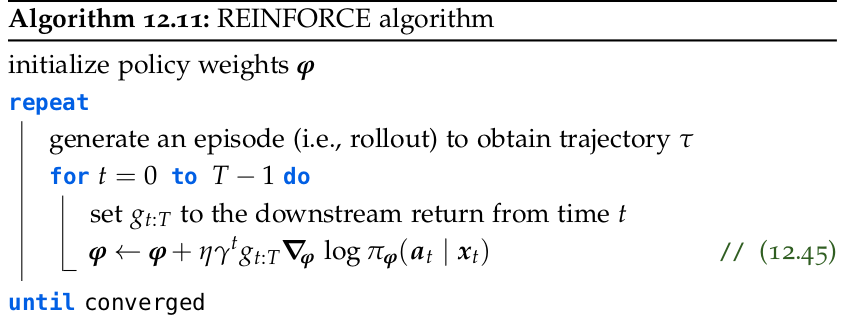
\includegraphics[width=\linewidth]{images/REINFORCE.png}
\begin{framed}
    Given a policy $\pi$, the \textbf{advantage function} is $\a[\pi]{\vx}{\va} \defeq \q[\pi]{\vx}{\va} - \v[\pi]{\vx} = \q[\pi]{\vx}{\va} - \E[\vap \sim \pi(\vx)]{\q[\pi]{\vx}{\vap}}$
\end{framed}
$\text{$\pi$ is optimal} \iff \forall \vx \in \spX, \va \in \spA : \a[\pi]{\vx}{\va} \leq 0$
\begin{framed}
    \textbf{Policy Gradient Theorem}\\
    The policy gradient can be represented in terms of the Q-function: \(\grad_{\varphi}{j(\varphi)}=\sum_{t=0}^{\infty}{\mathbb{E}_{\vx_t,\va_t}[\gamma^t q^{\pi_\varphi}(\vx_t,\va_t)\grad_\varphi \log \pi_{\varphi}(\va_t\mid \vx_t)]}\).

    
\end{framed}
\begin{framed}
  \textbf{Actor-Critic methods} consist of two components: a parameterized policy, $\pi(\va \mid \vx; \vvarphi) \eqdef \pi_\vvarphi$, which is called \textbf{actor}; and a value function approximation, $\q[\pi_\vvarphi]{\vx}{\va} \approx \Q[\pi_\vvarphi]{\vx}{\va; \vtheta}$, which is called \textbf{critic}.
\end{framed}
%Use gradient approximation: 
%\tiny{$\grad_\vvarphi \J{\vvarphi} \approx \sum_{t=0}^\infty\E[(\vx_t,\va_t) \sim \pi_\vvarphi]{\gamma^t \Q{\vx_t}{\va_t; \vtheta} \grad_\vvarphi \log \pi_\vvarphi(\va_t \mid \vx_t)}$}
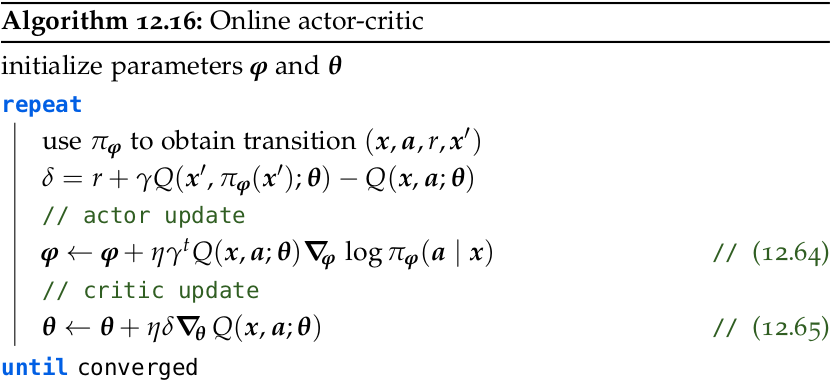
\includegraphics[width=0.95\linewidth, trim={0 0 4cm 0}, height=2.5cm]{images/Online_actor_critic.png}
\begin{framed}
    \textbf{Maximum Entropy Reinforcement Learning}
    Encourage exploration by regularizing policies towards uncertainty: \(j_{\lambda}(\varphi)=j(\varphi)+\lambda \H{\Pi_{\varphi}}\).
\end{framed}
